\documentclass[unicode]{beamer}
\usetheme{Copenhagen}
\usepackage{luatexja,tikz}% japanese
\usetikzlibrary{cd}
\usepackage[ipaex]{luatexja-preset}% IPAex font
\usecolortheme[RGB={15,95,125}]{structure}
\usefonttheme{professionalfonts} %font of mathematical formula
\usepackage{mlmodern}%thick math font 

\title{タリラリランのコニャニャチワ}
\subtitle{tarirariran}
\author{sanbon}
\institute{chuo junior high school}
\subject{}
\begin{document}
	\begin{frame}{how to use beamer}
		\titlepage
	\end{frame}
	
	\begin{frame}{hello}
		\begin{block}{block}
			This environment is block
		\end{block}

		\begin{alertblock}{alertblock}
			This environment is alertblock
		\end{alertblock}

		\begin{exampleblock}{exampleblock}
			This environment is exampleblock
		\end{exampleblock}
	\end{frame}

	\begin{frame}{mathematical formula}
	\[ \int^\infty_{-\infty}\frac{1}{\sqrt{2\pi}}e^{-\frac{x^2}{2}} dx \]
	\end{frame}

	\begin{frame}[fragile]{tikz}
		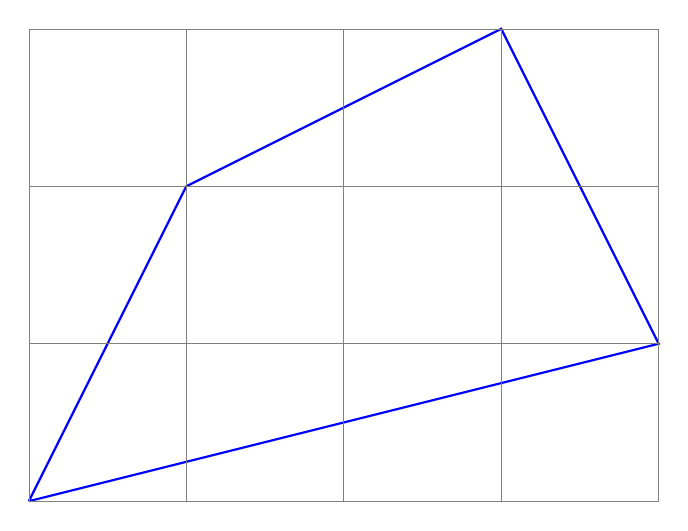
\begin{tikzpicture}[scale=2]
			\draw[color=blue,thick] (0,0) -- (1,2) -- (3,3) -- (4,1) -- (0,0);
			\draw[help lines] (0,0) grid (4,3);
		\end{tikzpicture}
		
	\end{frame}


	\begin{frame}[fragile]{commutative diagram}%fragile option is needed when you use tikz with beamer
		\begin{block}{five lemma}
			\[ 
				\begin{tikzcd}
					M_1 \arrow[r,"f_1"]\arrow[d,"h_1"] & M_2 \arrow[r,"f_2"]\arrow[d,"h_2"] & M_3 \arrow[r,"f_3"]\arrow[d,"h_3"] & M_4\arrow[r,"f_4"]\arrow[d,"h_4"] & M_5 \arrow[d,"h_5"]\\
					N_1 \arrow[r,"g_1"] & N_2 \arrow[r,"g_2"] & N_3 \arrow[r,"g_3"] & N_4\arrow[r,"g_4"] & N_5 \\
				\end{tikzcd}
		\]
		\vspace{-35pt}
		\begin{enumerate}
			\item[(1)]
				$h_1\colon$ surjection, $h_2,h_4\colon$injection$\Longrightarrow h_3\colon $injection
			\item[(2)]
				$h_5\colon$ surjection, $h_2,h_4\colon$surjection$\Longrightarrow h_3\colon $surjection
			\item[(3)]
				 $h_1,h_2,h_4,h_5\colon$bijection$\Longrightarrow h_3\colon $bijection
		\end{enumerate}
		\end{block}
	\end{frame}
	\begin{frame}[fragile]{five lemma}
			\[ 
				\begin{tikzcd}
					M_1 \arrow[r,"f_1"]\arrow[d,two heads,"h_1"] & M_2 \arrow[r,"f_2"]\arrow[d,hook,"h_2"] & M_3 \arrow[r,"f_3"]\arrow[d,"h_3"] & M_4\arrow[r,"f_4"]\arrow[d,hook,"h_4"] & M_5 \arrow[d,"h_5"]\\
					N_1 \arrow[r,"g_1"] & N_2 \arrow[r,"g_2"] & N_3 \arrow[r,"g_3"] & N_4\arrow[r,"g_4"] & N_5 \\
				\end{tikzcd}
		\]
		Let $x$ be a element of $\ker h_3$. If $x=0$,then $h_3$ is injective.
	\end{frame}
\end{document}
